\documentclass[a4j,12pt,twoside]{jreport}

%%%%%%%%%%%%%%%%%%%%%%%%%%%%%%%%%%%%%%%%%%%%%%%%%
% パッケージ宣言
%%%%%%%%%%%%%%%%%%%%%%%%%%%%%%%%%%%%%%%%%%%%%%%%%
\usepackage{graphicx}
\usepackage{times}
\usepackage{selectp}
\usepackage{epsf}
\usepackage{styles/epsbox}
\usepackage{styles/mediabb}
%\usepackage{styles/boites_exemples}
\usepackage{styles/verbatimfiles}
\usepackage{here}
\usepackage{url}
\usepackage{fancyhdr}
\usepackage{fancyvrb}
\usepackage{styles/algorithm}
\usepackage{styles/algorithmic}
\usepackage{cite}
\usepackage[dvipdfmx, usenames]{color}
\usepackage{colortbl}

\usepackage{ascmac}
\usepackage{amsmath}
\usepackage{amsthm}
\usepackage{amssymb}
\usepackage{latexsym}

\usepackage{styles/thesis}

%%%%%%%%%%%%%%%%%%%%%%%%%%%%%%%%%%%%%%%%%%%%%%%%%
% マクロ定義
%%%%%%%%%%%%%%%%%%%%%%%%%%%%%%%%%%%%%%%%%%%%%%%%%
\newcommand{\argmax}{\mathop{\rm argmax}}
\newcommand{\argmin}{\mathop{\rm argmin}}
\renewcommand{\bibname}{参考文献}

%% myマクロ
%\input{mymacros}

%% マージン設定
%\oddsidemargin=17mm
%\evensidemargin=-4mm

%%%%%%%%%%%%%%%%%%%%%%%%%%%%%%%%%%%%%%%%%%%%%%%%%
% 本文開始
%%%%%%%%%%%%%%%%%%%%%%%%%%%%%%%%%%%%%%%%%%%%%%%%%
\begin{document}
\newtheorem{defi}{Definition}[section]
\newtheorem{thy}{Theorem}[section]

\pagestyle{fancyplain}

\newlength{\oldtextwidth}
\setlength{\oldtextwidth}{\textwidth}
\setlength{\textwidth}{40zw}

% タイトル
%!TEX root = ../../main.tex
% タイトルページ
%\documentclass[a4j,12pt]{jreport}
%\usepackage{graphicx}
%\usepackage{times}
%\usepackage{selectp}
%\usepackage{epsf}
%\usepackage{epsbox}
%\usepackage{graphicx}
%\usepackage{verbatimfiles}
%\usepackage{here}
%%\usepackage{url}
%\usepackage{fancyhdr}
%\usepackage{algorithm}
%\usepackage{cite}
%\usepackage{ascmac}
%\usepackage{amsmath}
%\usepackage{amsthm}
%\usepackage{amssymb}
%\usepackage{latexsym}

%\usepackage{thesis}
%\input{mymacros}

%\oddsidemargin=17mm
%\evensidemargin=-4mm

%\setlength{\textwidth}{40zw}
%\begin{document}

\thispagestyle{empty}
\setcounter{page}{0}

%%%%%%%%%%%%%%%%%%%%%%%%%%%%%%%%%%%%%%%%%%%%%%%%%
% 定義
%%%%%%%%%%%%%%%%%%%%%%%%%%%%%%%%%%%%%%%%%%%%%%%%%

% タイトル
\def \title{MissionForest: 組織内外における\\協働支援のためのタスク構造化システムの試作}

% 著者
\def \author{後藤~誉昌}

% 提出日
\def \date{\today}

% 指導教官名
\def \teacher{白松~俊}

% 指導教官の肩書き
\def \teacherrank{准教授}

% 所属
\def \belong{名古屋工業大学\\工学部 情報工学科}

% 入学年度
\def \year{23}

% 学籍番号
\def \regnum{24115054}

%%%%%%%%%%%%%%%%%%%%%%%%%%%%%%%%%%%%%%%%%%%%%%%%%
% 本文
%%%%%%%%%%%%%%%%%%%%%%%%%%%%%%%%%%%%%%%%%%%%%%%%%

\def\sizeLL#1{\Huge #1}
\def\sizeL#1{\LARGE #1}
\def\sizeM#1{\Large #1}
\def\sizeS#1{\large #1}

\def\REYrule{\hbox to 5cm{\leaders\hrule height 1pt\hfill}}
\newbox\REYbox
\def\announce#1{
  \setbox\REYbox=\hbox{\REYrule\quad{\Large\bf #1}\quad\raise3pt\REYrule}%
  \gdef\REYbigrule{\hbox to \wd\REYbox{\leaders\hrule height 1pt \hfill}}%
  \centerline{\raise3pt\REYrule\vspace*{2mm}\quad{\LARGE #1}\quad\raise3pt\REYrule}}
\def\endannounce{\par\centerline{\REYbigrule}}

\begin{titlepage}
 \begin{center}
 %\renewcommand{\baselinestretch}{1.0}
  \vspace*{5mm}
  \sizeLL{卒業論文}\\
  \vspace*{10mm}
  \begin{announce}{(題~~目)}
   \sizeL{\title}\\
  \end{announce}
  \vspace*{20mm}
  \sizeM{指導教員~~~~~}\sizeL{\teacher}\sizeM{~~\teacherrank}\\
  %\vspace*{40mm} % 題目が2行の場合
 % \vspace*{30mm} % 題目が3行の場合
 \vspace{10mm}
  \sizeM{\belong}\\
  \vspace*{10mm}
  \sizeM{平成 \year 年 4 月 入学}\\
  \vspace*{3mm}
  \begin{table}[H]
    \begin{center}
     \begin{tabular}{cl}
      \sizeM{(学籍番号)} & \sizeL{{\underline{~~ \regnum ~~}}} \\
      \sizeM{(氏~名)} & \sizeL{\underline{~~ \author ~~}} \\
     \end{tabular}
    \end{center}
   \end{table}
  \vspace*{10mm}
  \sizeS{(提出日:~\today)}
  % \sizeS{(提出日:\ ~平成28年2月8日)}
 \end{center}
\end{titlepage}

%\end{document}

\cleardoublepage

% タイトル以降用パラメータ
\setlength{\oddsidemargin}{17mm}
\setlength{\evensidemargin}{-4mm}
\setlength{\textwidth}{\oldtextwidth}

\cleardoublepage

%ここからページ数開始
\pagenumbering{arabic}
\cleardoublepage

% アブストラクト
%!TEX root = ../../main.tex
\chapter*{論文要旨}
\label{chap0}
\addcontent{論文要旨}
本研究ではこれまで,公益活動やシビックテックといった分野を対象とし,公共圏で目標を共有するWebシステム「ゴオルシェア」[1]を開発・運営してきた.
従来のゴオルシェアは組織横断的な協働を想定しており,目標データを全てオープンデータ化していた.
しかし,組織内での日常的な活動は公開に適さないものも多いため,日常的には使いにくいという問題点があった.
また,目標を階層化したツリー構造の入力操作が直感的でないという問題点もあった.
そこで本稿で試作する新システム「MissionForest」では,(1)組織内部の日常的な活動を非公開な目標ツリーとして記録し,(2)外部発表後にツリー構造の一部をオープンデータ化可能にする.
さらに,(3)目標ツリーを直感的操作で作成・編集可能にする.

\cleardoublepage

% 目次
% 目次
\markboth{目 次}{目 次}
\tableofcontents

% 図目次
\listoffigures
\markboth{図 目 次}{図 目 次}

% 表目次
\listoftables
\markboth{表 目 次}{表 目 次}

\cleardoublepage

% 第1章 序論
%!TEX root = ../../main.tex
\chapter{序論}
\label{chap:intro}

\section{本研究の背景}
大学の研究室では,教員の指示だけに頼らず主体的に考えて研究できる学生の育成が求められている.
しかし研究生活に慣れていない学生にとってはうまく研究が進まないことも多く,また教員も逐一フォローアップできていない現状がある.
そこで,「どのような課題をどのようなアプローチで解決しようとしているか」を日常的に学生自身がデータ化し共有することで,教員や他学生とのコミュニケーションを支援し,
協働を促進することができると考える.

\section{本研究の目的}
学生の研究目標を公開・共有することによって,教員による進捗の把握や,学生の自律性向上,学生同士の協働の促進を目的としている.
また学外に対しても,研究アプローチや研究成果を公開することによって,外部組織との連携やアウトリーチ活動にも活用でき,公益活動にも研究シーズを活用できる可能性がある.

このようなシステムに必要になる要件は,(1)プロジェクト全体のタスクを俯瞰できる,(2)各タスクの進捗状況が把握できる,(3)各タスクに対して議論することができる,という3つを満たす必要がある.
このような要件を満たすシステムは”プロジェクト管理システム”と呼ばれ,有償無償問わず数多く存在する.
上記のような従来型のプロジェクト管理システムの機能に加え,プロジェクトの成果を公開することで,2次活用や外部組織との連携に役立てられることができれば,新たな協働を生む可能性がある.
そこで新システムMissionForestの試作により,新たな協働を生み,協働を支援できるようなプロジェクト管理システムを目指す.
プロジェクトの目標階層は,ゴオルシェアを踏襲してLinked Dataとして構造化した上で,ゴオルシェアよりも詳細に公開/非公開を制御できる機構を目指す.

\section{本論文の構成}
本論文の構成を以下に示す.
第2章では関連研究や関連システムと本研究の動作・開発環境について述べる.
第3章では直感的にツリーを作成できるインターフェースについて述べる.
第4章ではLODでの公開機構について述べる.
第5章では類似タスクの推薦機構について述べる.
第6章では前章までで述べたシステムの評価実験の結果をまとめる.
第7章で本研究をまとめる.

\cleardoublepage

% 第2章 動作・開発環境と関連研究
%!TEX root = ../../main.tex
\chapter{関連研究と動作・開発環境}
本章では本研究の関連研究と動作・開発環境について述べる.

\section{関連研究}
本研究と関連のある研究やシステムを紹介する.

\subsection{タスク階層構造}

\subsubsection{Work Breakdown Structure}
Work Breakdown Structure(WBS)とは,プロジェクトマネジメントで計画を立てる際に用いられる手法の一つで,プロジェクト全体を細かい作業に分割した構成図.
「作業分割構成」,「作業分解図」などとも呼ばれる.
WBSでは,まずプロジェクトの成果物をできるだけ細かい単位に分解していく.
その際,全体を大きな単位に分割してから,それぞれの部分についてより細かい単位に分割していき,階層的に構造化していく.
青果物の細分化が終わったら,それぞれの部分を構成するのに必要な作業を考え,最下層に配置していく.

\subsubsection{前提条件ツリー}
前提条件ツリー(Prerequisite Tree)\cite{zentei}の構成要素には,実現すべき目標と中間目標,そして目標を実現する上での障害がある.
前提条件ツリーで扱う関係は必要関係と克服関係である.
必要関係では,上位の目標を実現するためには下位の目標が必要であることを表す.
これに対して克服関係では上位の目標の障害を下位の中間目標によって解決できることを表す.
新たなシステムが成功するための前提条件を予め明らかにするために作成するのが前提条件ツリーである.

\subsection{プロジェクト管理システム}

\subsubsection{ゴオルシェア}
ゴオルシェア\cite{shiramatsu2016}とは,社会課題とその解決目標,さらにその部分目標をLOD化して共有するためのWebサービスである.
「誰がどんな課題に注目しているのか」「誰が何を目指して動いているのか」を一般市民が自ら入力して共有することで,
方向性の似た潜在的協力者を探すことができ,さらに有力者の目標を共有し,近未来社会像の透明性向上を図る.
LODの枠組みによって,社会課題と解決目標の関係や,その部分目標との関係,協力者との関係などを紐付けし,似た目標を探せるようにした.
多くの利害関係者が絡む社会問題を解決するためには,組織横断的な協働が不可欠であり,
従来のSNSには方向性の似た潜在的協力者を探す機能がなかったので,このようなシステムがあれば,
(1) 身の回りの社会課題や目指す目標を一般市民が公開&共有して,似た方向性の人々を探せるようにする,
(2) 断片的なニュースから,社会課題や有力者の目標を抽出&共有して,世の中の動きの透明性を向上させる,
ことができる.

\subsubsection{ナレッジコネクター}
ナレッジコネクター(Knowledge Connector)は,全国的に行われているオープンデータを活用したイベントの成果等を集約し
,一元的に検索を可能にするとともに,アイディアやアプリを創出した人材とビジネスパートナーとのマッチングを支援するためのサイト.
同じような課題を抱えている人,何かをやりたいと思っているが何から手をつけていいかわからない人,もしかしたら連携できる人やコミュニティを見つけることができる.

\subsubsection{みらいらぼ}
みらいらぼ\cite{sengoku2016}とは,共創の場を支援する集合知プロジェクト支援システムである.
みらいらぼは,Webアプリケーションであり,Web上でプロジェクトの作成,共有,およ ゙共創をすることができる.
また,みらいらぼはSNSとの連携が可能であり,多くの多様な人たちとプロジェクトの共有を行うことができ,集合知を用いてプロジェクトを進めることができる.
さらに,Web上だけでなく学会と合わせてみらいらぼを使うことによって,より共創を起こすことが可能である.

\subsection{合意形成システム}

\subsubsection{COLLAGREE}
COLLAGREE\cite{ito2016}とは,離れた場所にいる人々がweb上での議論を通して合意形成をはかるシステムである.
投稿されたつぶやきがシステムによって意見集約され,合意形成を行います.
限られた人々が一室に集まって行う従来の閉じられた議論ではなく,多くの人々がいつでもインターネット上で開かれた議論を行えることを目指している.

\section{動作・開発環境}

\subsection{Ruby}
Ruby\footnote{https://www.ruby-lang.org}は,まつもとゆきひろ氏により開発され,1995年12月にfj上で発表されたオブ
ジェクト指向スクリプト言語である.機能として,クラス定義,ガベージコレクション,
強力な正規表現処理,マルチスレッド,例外処理,イテレータ・クロージャ,Mixin,演
算子オーバーロードなどがある..Rubyにおいては整数や文字列なども含めデータ型は
すべてがオブジェクトであり,純粋なオブジェクト指向言語といえる.

\subsection{Ruby on Rails}
Ruby on Rails\footnote{http://rubyonrails.org}はデンマークのDavid Heinemeier Hanssonにより作成されたフレーム
ワークで,2004年7月に公開され,2005年12月13日にバージョン1.0がリリースされた.
Ruby on Railsは,フレームワークとしては一般的なMCV型に属する.MCV型とは,
Model-View-Controllerの頭文字をとった言葉で,データとそれに関わる処理を担う「モ
デル(Model)」,表示・出力を行う「ビュー(View)」,これらのビューとモデルを制御す
る「コントローラー(Controller)」といった3つのコンポーネントを基礎とするアーキテ
クチャである.このように機能を分割しておくと,ビュー・コントローラーとモデルが疎
結合になることによってモデルの再利用性が高まり同時にビューの入れ替えが容易にな
り,ソースコードの見通しもよくなる.
Ruby on Railsには,基本理念として「同じことを繰り返さない」(DRY:Don't Repeat
Yourself)と「設定よりも規約」(CoC:Convention over Configuration)がある.「同じこ
とを繰り返さない」(DRY)というのは,Andrew Hunt氏とDevid Thomas氏が打ち出した
原則で,定義などの作業は一回だけですませ,冗長なだけでなく往々にして間違いの元に
なる,重複や繰り返しを避けろという意味である.「設定よりも規約」(CoC)とは,Ruby
on Rails発祥の哲学で,レアなケースをも想定して冗長になりがちな設定を極力排除し,
規約に従うことでお決まりの動作を実現させようという思想である.
また,Ruby on Railsはフレームワークであるだけでなく開発環境でもある.Ruby on
Railsには,コード生成機能があり,基本理念の1つである「設定よりも規約」に基づく
テンプレートが配置され,通常1画面ごとに手作業で用意していたスケルトンがスクリプ
ト1つで生成でき,また,データベースレコードの新規作成,参照,更新,削除を行うよ
うな単純なWebアプリケーションもまたスクリプト1つで生成できる.さらに,Ruby on
Railsに用意されているのはコード生成機能だけではなく,すぐに動かして試せる簡易
Webサーバやインタラクティブシェルといったスクリプト,コード生成時にはテストコー
ドのひな型も同時に生成さる.これらにより,Webアプリケーションの開発が容易にな
る.

\subsection{MySQL}
MySQL(マイエスキューエル)\footnote{https://www.mysql.com}は,オープンソースで公開されている関係データベース管理システム (RDBMS) の一つである.
データベースでデータを操作する際には,「SQL」という言語を使う.
データの追加,削除,変更,検索などを行うだけでなく,データベースの構造やデータ型を定義する言語でもある.
他には PostgreSQL,Oracle などがある.
MySQLは他言語と比べ,処理速度が速く,非常に多くのデータを扱えるので,広い範囲での応用が可能である.
また,C,Java,Perl,PHP,Ruby など様々なプログラミング言語と接続可能で,多言語対応で,日本語は,SJIS,EUC ともにサポートしている.

\subsection{Stardog}
Stardog(スタードッグ)\footnote{http://stardog.com}は,Javaで書かれた有償のRDFストア.
推論エンジンPalletを開発するなど,セマンティック技術開発分野での実績があるComplexible社による製品.
特徴として,OWL2での推論や,ルール言語SWRLに対応している.
また,セキュリティ関連機能を持ち,データベースとユーザーそれぞれについてアクセス権を設定できる.
API経由での利用も可能である.

\cleardoublepage

% 第3章 直感的にツリーを作成できるインターフェース
\chapter{直感的にツリーを作成できるインターフェース}
先行研究である「ゴオルシェア」では,システムを直感的に操作することが難しかった.
本研究では,初めて使う人でも直感的に操作できるインターフェースを目指した.

\section{画面構成}
本システムの画面構成を,スクリーンキャプチャと共に以下に示す.

\subsection{ミッション一覧}
作成されたミッション一覧を閲覧できる画面を\ref{img:interface_capture_list}に示す.
ミッションはカード型に,タイトルと作成者を閲覧することができる.

\begin{figure}[t]
	\begin{center}
		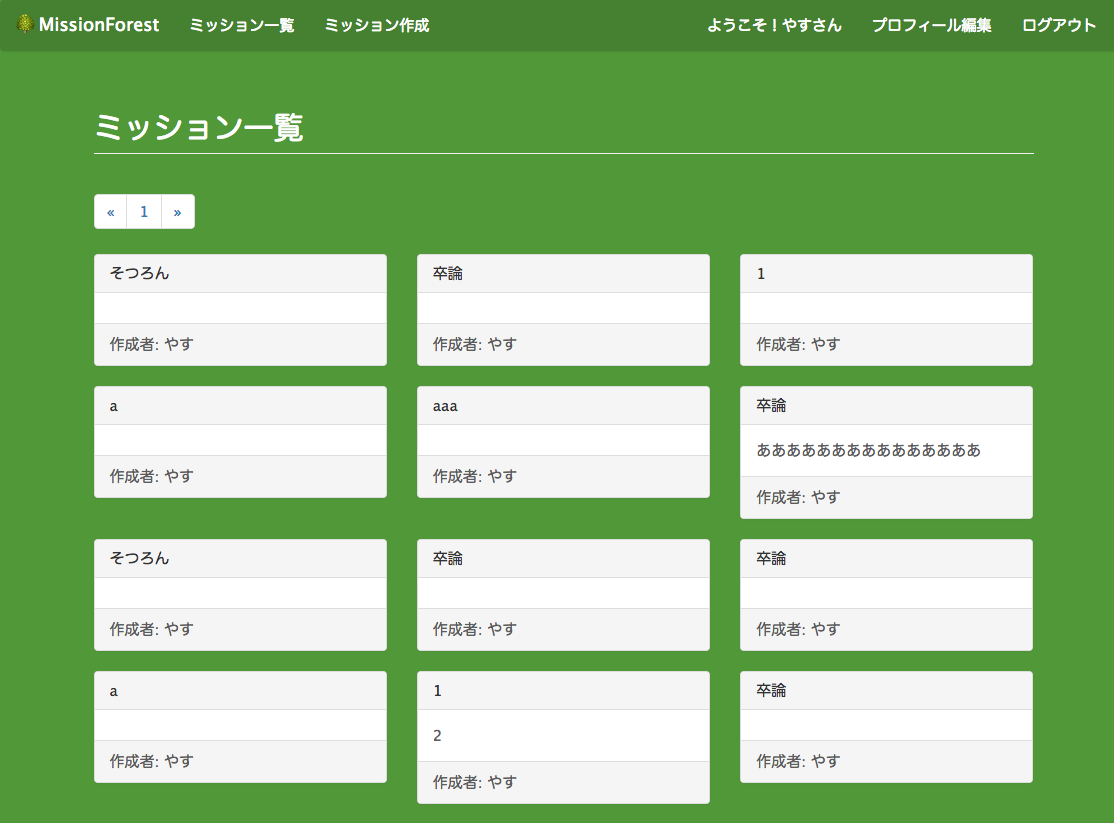
\includegraphics[width=0.9\linewidth]{assets/img/interface_capture_list.png}
		\caption{動作画面}
		\label{img:interface_capture_list}
	\end{center}
\end{figure}

\subsection{ミッション詳細}
ミッションの詳細画面を\ref{img:interface_capture_detail}に示す.
ミッションのタイトル,作成者,概要とともに,ミッションツリーを閲覧することができる.

\begin{figure}[t]
	\begin{center}
		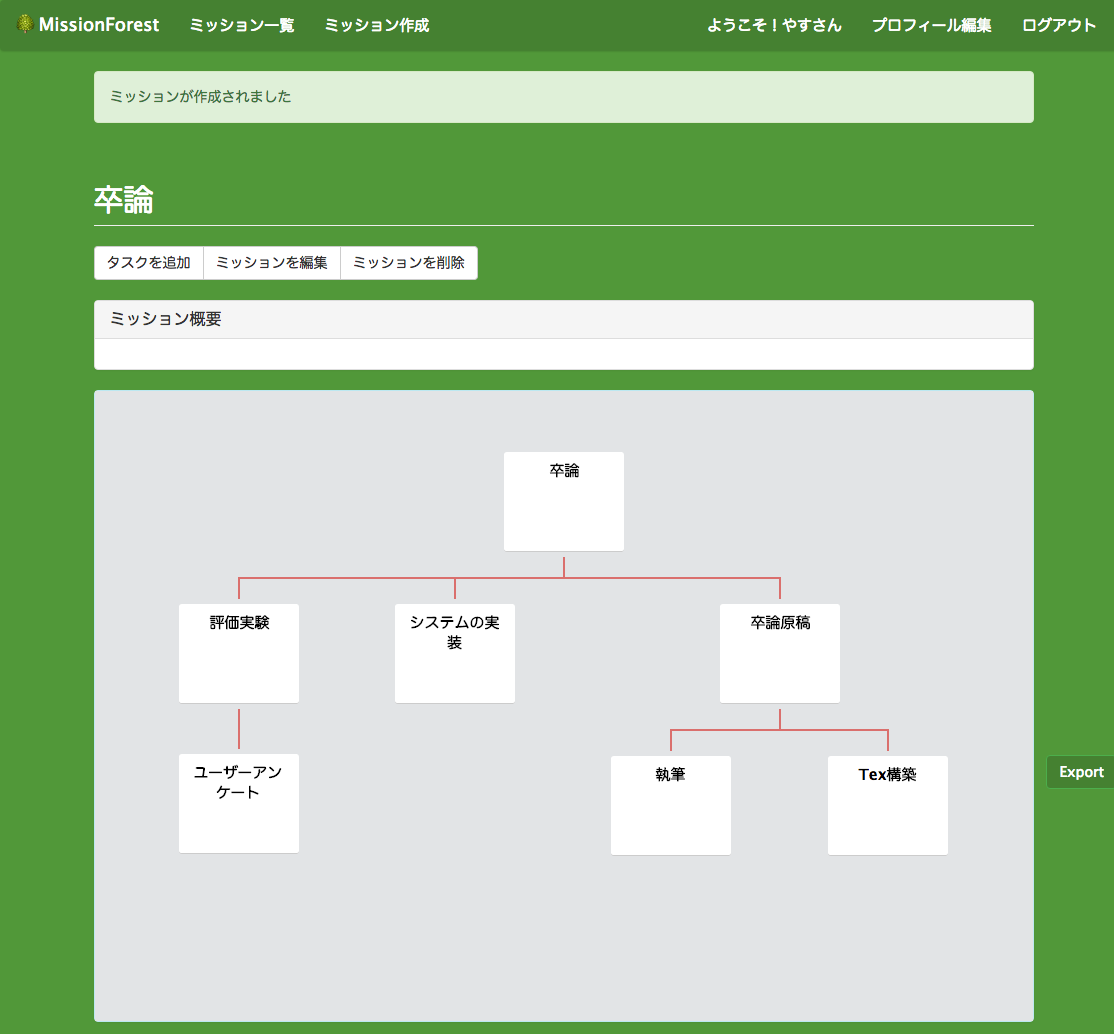
\includegraphics[width=0.9\linewidth]{assets/img/interface_capture_detail.png}
		\caption{動作画面}
		\label{img:interface_capture_detail}
	\end{center}
\end{figure}

\subsection{タスク追加}
タスクの追加画面を\ref{img:interface_capture_add}に示す.
タスクをクリックするとその子タスクを追加するモーダルが表示され,タスク名,概要,締め切りを入力することができる.

\begin{figure}[t]
	\begin{center}
		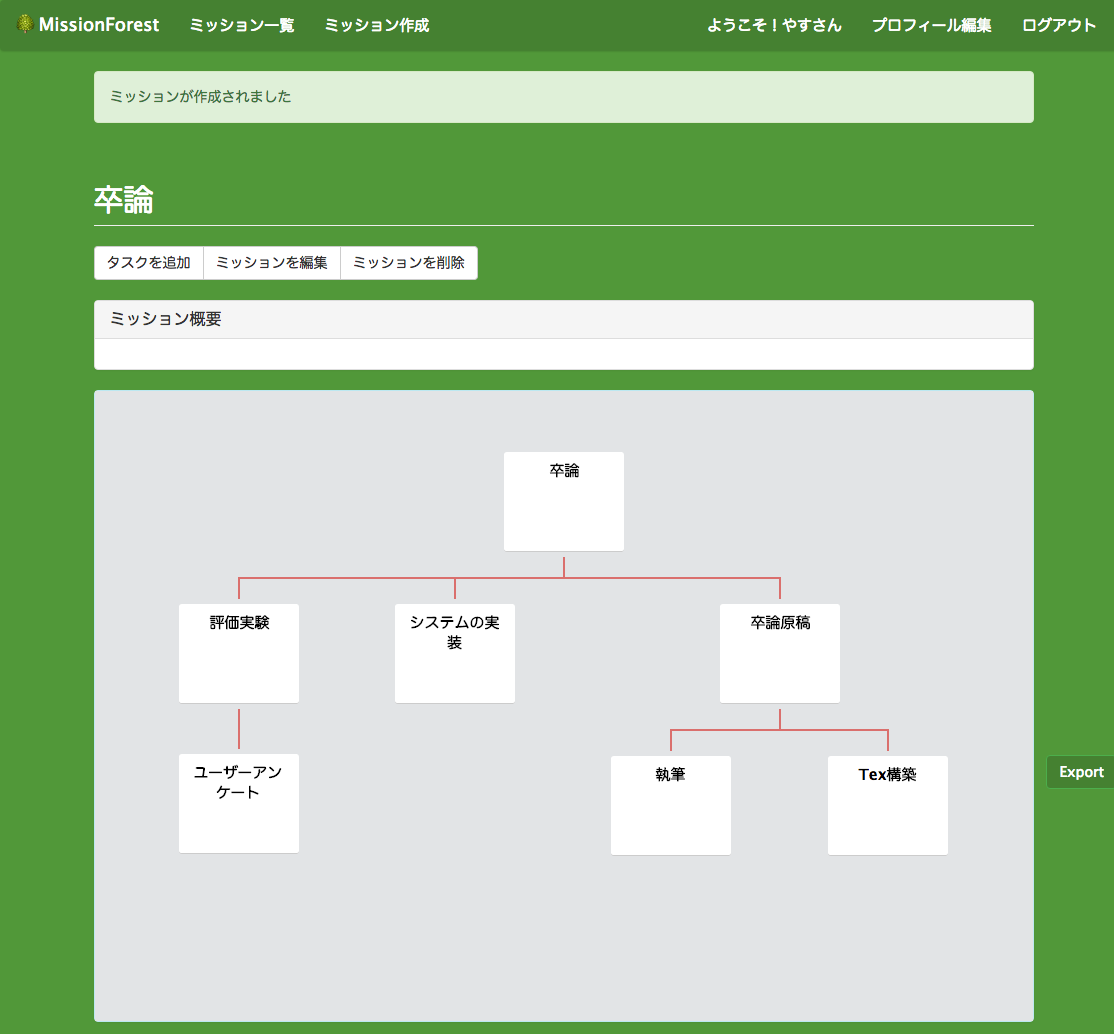
\includegraphics[width=0.9\linewidth]{assets/img/interface_capture_add.png}
		\caption{動作画面}
		\label{img:interface_capture_add}
	\end{center}
\end{figure}

\section{アプリケーション}
\subsection{Ajaxによる非同期通信}
従来のシステムでは,タスクを追加するたびにページ読み込みが発生し,1つのミッションを完成させるのに時間がかかっていた.
またページ読み込みされてしまうので,自分がどのタスクを編集していたのかが分かりづらかった.
そこで,本システムではAjaxを用いた非同期通信を用いることで,ページ読み込みなしにタスク追加をすることができるようにした.
また,サーバーとの通信は適切なデータのみをJSON形式でやり取りするので,レスポンスも向上した.

\subsection{システム構成}
本システムのシステム構成を図\ref{img:system_architecture}に示す.
まずプロジェクトを閲覧する場合,Webブラウザから非同期通信によってWebAPIにアクセスする.
WebAPIはメインデータベースであるMySQLからユーザー認証情報,ミッションやタスクの情報を取得し,JSON形式でレスポンスを返す.
次にプロジェクトを投稿する場合,Webブラウザから非同期通信によってWebAPIにJSON形式でデータをPOSTし,WebAPIはメインデータベースであるMySQLに受け取ったデータを保存する.
さらに,タスクごとに設定されたアクセス権限によって,RDFストアであるStardogにLODとして保存する.

\begin{figure}[t]
	\begin{center}
		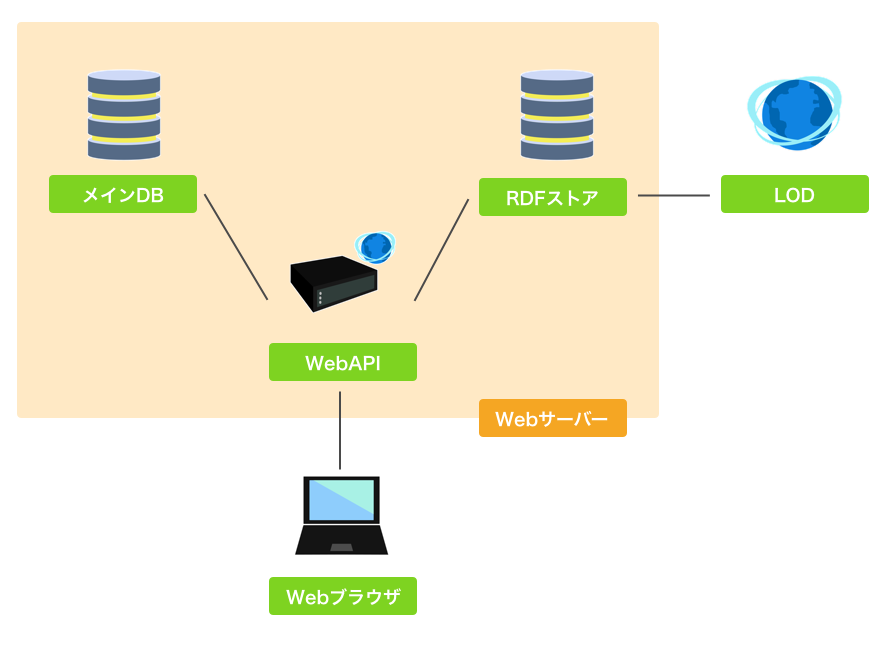
\includegraphics[width=0.9\linewidth]{assets/img/system_architecture.png}
		\caption{システム構成図}
		\label{img:system_architecture}
	\end{center}
\end{figure}

\section{主な機能}
試作するシステムでは,プロジェクトを「ミッション」と呼ぶ.
ユーザーは任意にミッションを作成することができ,ミッションごとに直感的なGUIでタスクツリーを構築することができる.
タスクには進捗状況の指定,タグの指定,コメント機能,編集履歴,ファイル添付をすることができる.
作成したミッションは任意のタイミングで一般公開することができるので,公開されたミッション間から後述するアルゴリズム類似ミッションを推定し,ユーザーに推薦することにより,組織を越えた協働を促進する.

\section{ツリーエディタ}
直感的なツリーエディタGUIを作成するため,本研究で使用したJavaScriptライブラリを述べる.

\subsection{実装手法}
dabengが開発したOrgChart\footnote{https://github.com/dabeng/OrgChart}というjQueryライブラリをベースに拡張し,ミッションツリーを表現している.
このOrgChartでは,タスクのレイアウトに,HTMLのテーブル機能を用いている.
具体的には,HTMLのテーブル属性(<table>)は,カラム(<td>)の要素数に応じて列の幅が均等にレイアウトされる.
この性質を用い,1階層を1テーブルとみなし,テーブルのカラムの中にテーブルをネストすることで,HTMLにより再帰的にすべてのカラムが等間隔に配置される.

また先ほど述べたように,Ajaxを用いた非同期通信をするために,ツリーに表示するデータはAPIから\ref{img:json_sample}に示すようなJSON形式で取得している.
タスクの追加,編集,削除があった場合は,このデータとなるJSONが変更されるので,ツリーエディタ上も変更される.

\begin{figure}[t]
	\begin{center}
		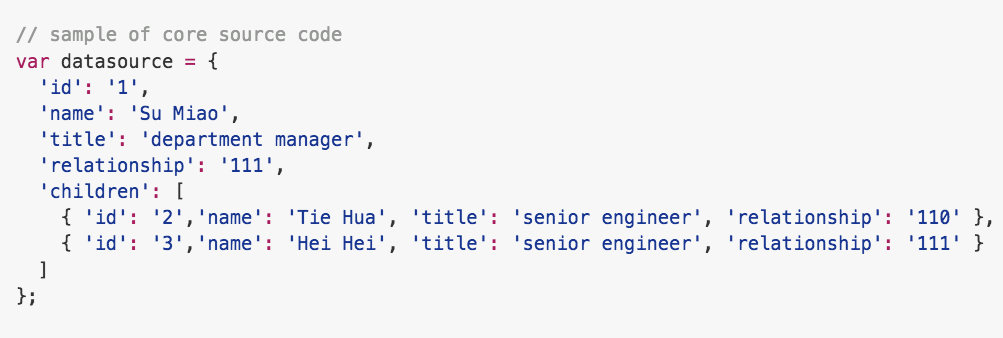
\includegraphics[width=0.9\linewidth]{assets/img/json_sample.png}
		\caption{システム構成図}
		\label{img:json_sample}
	\end{center}
\end{figure}

\cleardoublepage

% 第4章 LODでの公開機構
\chapter{LODでの公開機構}
本章ではLODでの公開機構について述べる.

\section{4つのアクセス権限}
先に述べたように,ゴオルシェアではLinked Dataのアクセス権限を指定することができず,自動的にすべてのデータが誰でも閲覧できる状況にあった.
しかし研究室など限られた組織内で使うには,アクセス権限のあるユーザーのみが閲覧できる仕組みが必要である.
そこで現状では,アカウント単位でのアクセスコントロール機能があるRDFストアであるStardogを用いて,表1に示すような,プロジェクトの段階に応じたアクセス制御機構を実装中である.
具体的には\ref{img:permission_table}に示すように,(1)プロジェクトが個人的な構想段階である初期場合,(2)組織内限定で共有される段階,(3)外部発表後に外部公開する段階,(4)オープンライセンスで公開し,組織横断的な協働を志向する段階,の4段階を想定し,各段階に応じたアクセス制御機構を想定している.
プロジェクトの段階が進んでいくにつれて,公開したいタスクが増えていくと考えられる.
ただし,より具体的な下層の葉に近いタスクは,段階が進んだとしても公開に適さない場合が多いと考えられる.
そこで,タスクツリーからユーザが公開したいタスクのみを部分的に選択できるようなインターフェースも必要となる.
このような公開箇所の選択機構についても,現在実装中である.

\begin{figure}[t]
	\begin{center}
		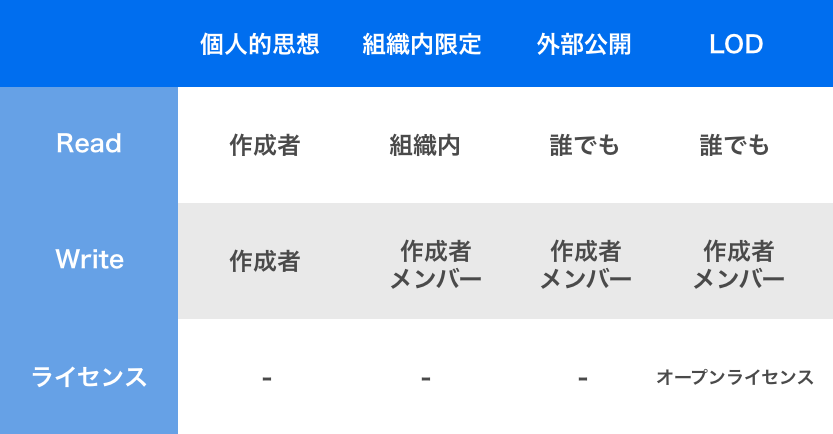
\includegraphics[width=0.9\linewidth]{assets/img/permission_table.png}
		\caption{アクセス権限}
		\label{img:permission_table}
	\end{center}
\end{figure}

\section{実装手法}
// TODO: 具体的な実装手法

\cleardoublepage

% 第5章 類似タスクの推薦機構
%!TEX root = ../../main.tex
\chapter{ユーザースキルの推薦機構}
本章ではユーザースキル推薦機構について述べる.

\section{スキルタグ}

\subsection{活用事例}
世界最大級のビジネス特化型ソーシャル・ネットワーキング・サービスであるLinkedIn\footnote{https://www.linkedin.com}や,
IT/Web業界最大級のソーシャル・リクルーティング・ツールであるWantedly\footnote{https://www.wantedly.com}や,
では,自分のスキルタグを登録することができる.
このスキルタグを用いて,ユーザー同士のマッチングをしたり,採用活動に活用している.

\section{ユーザースキルの推定}
本システムでは,そのタスクの完了に必要なスキルをタグとして設定することができる.
タスクに紐付いたスキル情報から,それぞれのユーザーが持っているスキルを推薦し,マッチングなどに活用することを今後の課題としている.

\subsection{推薦手法の検討}
タスクに紐付いたスキルから,ユーザーごとのスキルを推薦する手法について検討する.

\subsubsection{出現回数を用いる}
ユーザーが作成したすべてのタスクに紐付いているスキルのうち,登録された数が多いもの上位から推薦することで,たくさんこなしたスキルをユーザースキルとして推薦することができる.
この手法では,そのミッションではそのスキルを必要とするタスクが多かっただけで,そのユーザーが本当にそのスキルに精通しているかは不明である.

\subsubsection{タスク完了までの時間を用いる}
本システムでは,タスクにTODO・進行中・完了の3つの進捗状況を指定することができる.
またこれに加え,そのタスクの完了に必要な見積もり時間を設定できる機能を開発予定である.
この手法ではこれを用い,タスクの見積時間に対して実際にかかった時間が短かったものを上位として推薦することで,ユーザーの得意なスキルを推薦することができる.

\subsubsection{タスクの階層を用いる}
一般に,タスクの階層が深くなればなるほどより細かくタスク分解された具体的なタスクになる.
階層が深いタスクに紐づくスキルを上位として推薦することで,より具体的なスキルをユーザースキルとして推薦することができる.

\section{本システムでの活用の検討}

\subsection{アドバイザーの推薦}
そのミッションやタスクに関するスキルを有している人をアドバイザーとしてマッチングすることができる.
これにより,円滑にプロジェクトを進めることができる.

\subsection{チームビルディングでの活用}
ハッカソンなどのチームビルディングの場において,人的資源であるスキルの相補性が重要となる.
本システムのユーザースキルを用いることにより,スキルを補完しあったバランスの良いチームビルディングが可能になる.

\cleardoublepage

% 第6章 性能評価・考察
%!TEX root = ../../main.tex
\chapter{性能評価・考察}
本研究の評価として,システムの操作性と推薦機構の評価実験を行った.

\section{システムの操作性の比較実験}
先行研究であるゴオルシェアと,私が開発しているミッションフォレストとの,操作性の比較実験を行った.

\subsection{実験内容}
サンプルとして\ref{img:experiment_question}に示すプロジェクトを提示し,ゴオルシェア及びミッションフォレスト両システムで作成してもった.
実際に作成されたツリーを,\ref{img:experiment_goalshare}と\ref{img:experiment_missionforest}に示す.
ウェブユーザビリティ評価スケール(WUS)に基づく評価項目\ref{table:experiment_question}について,どちらのシステムがよかったか評価してもらった.

\begin{figure}[t]
	\begin{center}
		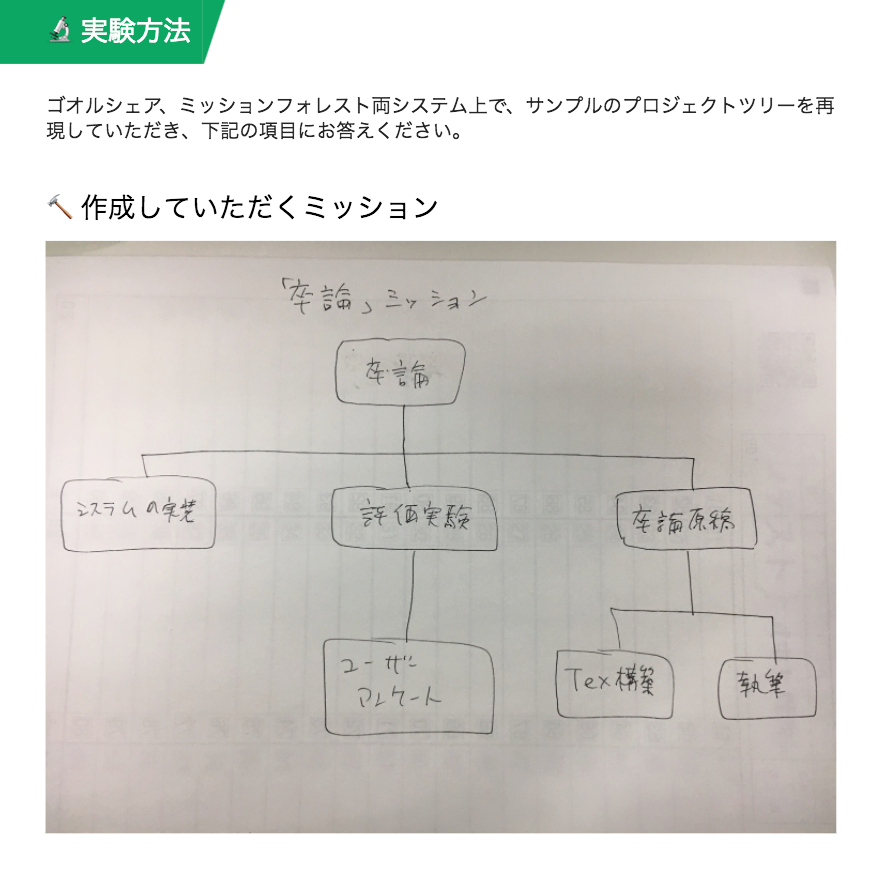
\includegraphics[width=0.9\linewidth]{assets/img/experiment_question.png}
		\caption{評価実験例題}
		\label{img:experiment_question}
	\end{center}
\end{figure}

\begin{figure}[t]
	\begin{center}
		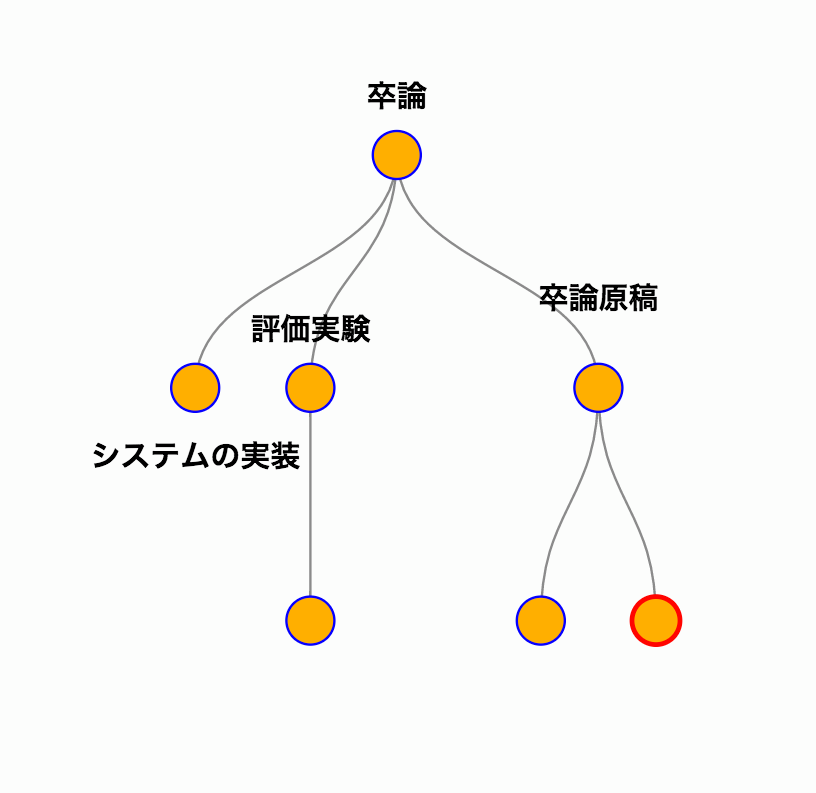
\includegraphics[width=0.9\linewidth]{assets/img/experiment_goalshare.png}
		\caption{ゴオルシェア実験結果}
		\label{img:experiment_goalshare}
	\end{center}
\end{figure}

\begin{figure}[t]
	\begin{center}
		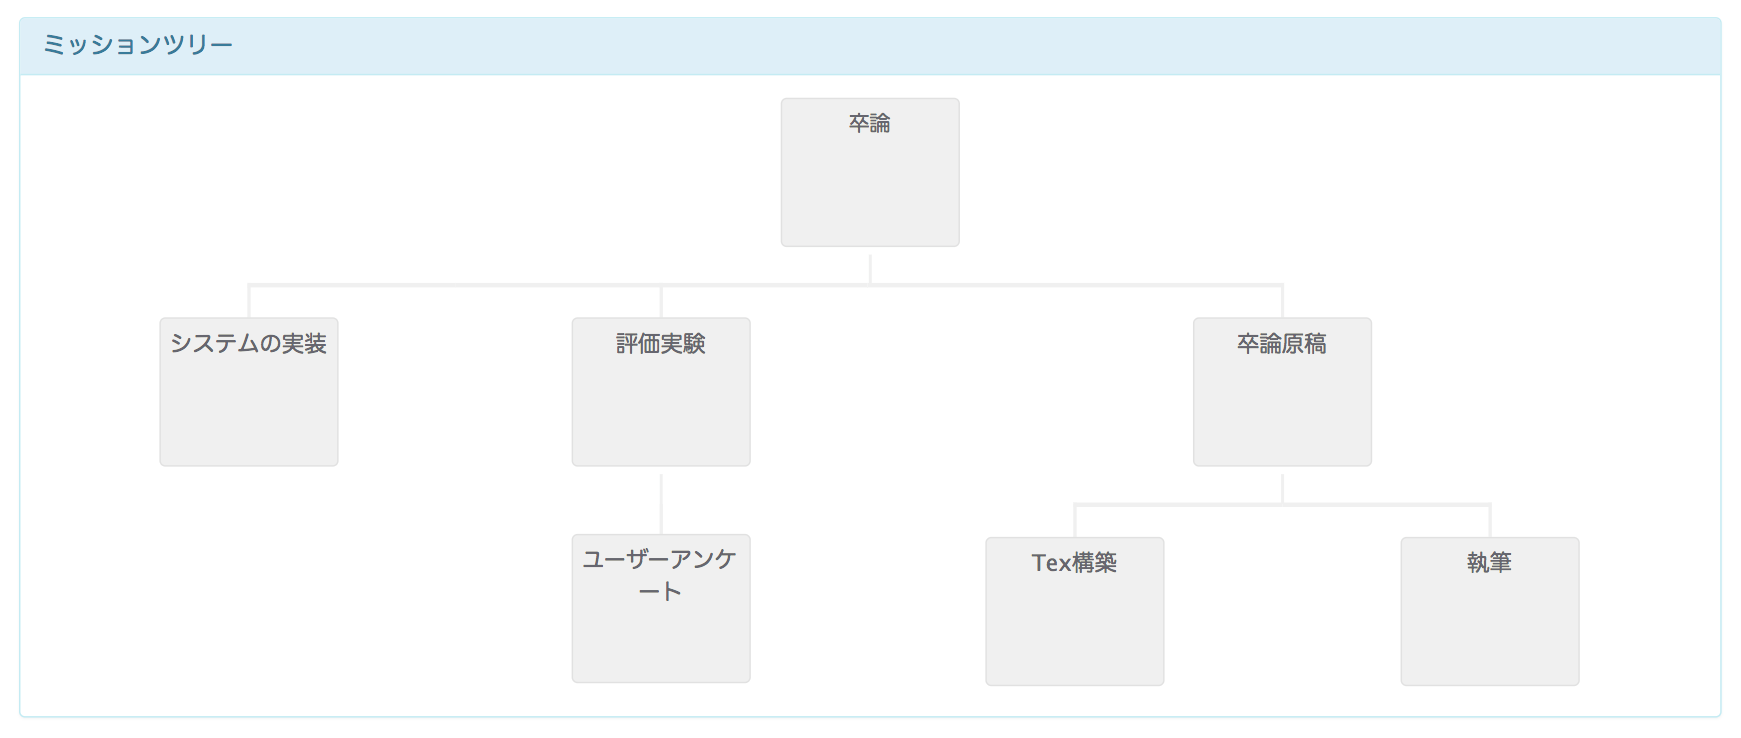
\includegraphics[width=0.9\linewidth]{assets/img/experiment_missionforest.png}
		\caption{ミッションフォレスト実験結果}
		\label{img:experiment_missionforest}
	\end{center}
\end{figure}

\begin{table}[t]
 \caption{評価実験項目}
 \begin{center}
	 \begin{tabular}{ | c | c | } \hline
			1 & ミッションの作成はどちらが操作しやすかったですか \\ \hline
 			2 & タスクの作成はどちらが操作しやすかったですか \\ \hline
 			3 & 画面上のUI構成はどちらがわかりやすかったですか \\ \hline
 			4 & どちらのツリー表示が見やすかったですか \\ \hline
 			5 & 軽快な動きをするのはどちらでしたか \\ \hline
 			6 & 今後どちらのシステムを使いたいですか \\ \hline
	 \end{tabular}
	 \label{table:experiment_question}
 \end{center}
\end{table}

\subsection{実験結果と考察}
今回はサンプルとして,10名の被験者に評価実験を行ってもらった.
以下に各評価項目ごとの結果と考察を述べる.

\subsubsection{(1)ミッションの作成はどちらが操作しやすかったですか}
TODO: エラーバーグラフ

\subsubsection{(2)タスクの作成はどちらが操作しやすかったですか}
TODO: エラーバーグラフ

\subsubsection{(3)画面上のUI構成はどちらがわかりやすかったですか}
TODO: エラーバーグラフ

\subsubsection{(4)どちらのツリー表示が見やすかったですか}
TODO: エラーバーグラフ

\subsubsection{(5)軽快な動きをするのはどちらでしたか}
TODO: エラーバーグラフ

\subsubsection{(6)今後どちらのシステムを使いたいですか}
TODO: エラーバーグラフ

\cleardoublepage

% 第7章 まとめ
%!TEX root = ../../main.tex
\chapter{まとめ}

\section{本研究の要約}
本稿では,タスクツリーを直感的ユーザインタフェースで編集可能であり,プロジェクトの段階を考慮したアクセス制御機構により部分的なオープンデータ化が可能なMissionForestの試作について述べた.
実装中であるアクセス制御機構および公開タスクの部分的選択機構については,実装が完了し次第,評価実験を行う予定である.

\section{今後の展望}
今後は,研究室内でのソースコード共有やハッカソンでの使用を想定し,GithubやSlackなどの外部サービスとの連携を可能にする.
また,Web議論システムCOLLAGREE [6]との連携による協働プロセスのアーカイブ化など,より実効性の高い協働支援のできるタスク構造化システムを開発していく予定である.

\cleardoublepage

% 謝辞
%!TEX root = ../../main.tex
\chapter*{謝辞}
\addcontent{謝辞}
本論文を執筆するにあたり,多くの方のご支援ご協力を賜りました.
この場で皆様に感謝の言葉を申し上げたいと思います.

まず,名古屋工業大学大学院 工学研究科 情報工学専攻の白松~俊准教授に厚く御礼申し上げます.
白松教授には日々の研究活動に限らず,研究経験の乏しい私に懇切丁寧にご指導して頂き,数多くの貴重な体験もさせて頂きました.
ここに心より感謝致します.

同研究室の同輩である成瀬~雅人君,西田~拓哉君,山野~太靖君とは特に苦楽を共にしてきました.
その中で,皆の頑張り,励まし,助言に助けられることも多く,充実した日々を過ごすことができました.
ここでみなさんに感謝の意を表しつつ,今後のご活躍をお祈り申し上げます.

最後に,研究活動で帰りが遅くなることもあり迷惑をかけた私を,いつもと変わらず支えてくれた家族に,心より感謝致します.

\vspace*{4.5mm}

\begin{flushright}
思い出で溢れている 白松研究室にて \\
2016年 桜咲く頃に \\
\vspace*{1.8mm}
\end{flushright}

\cleardoublepage

% 参考文献
%!TEX root = ../../main.tex
%修論用
% 参考文献 http://bibdesk.sourceforge.net/manual/BibDesk%20Help_94.html#SEC179 による出力
%以下テンプレ
%<$publications>
%\bibitem{<$citeKey/>}
%<$authors.name.stringByRemovingTeX.@componentsJoinedByComma/>: ``<$fields.Title.stringByRemovingTeX/>,''  <$fields.Journal.stringByRemovingTeX/>. Vol. <$fields.Volume/>,  No. <$fields.Number/>,  pp. <$fields.Pages/>,  <$fields.Year/>.
%<$fields.URL/>
%<$fields.localURL/>
%\begin{quote}
%\end{quote}

%
%</$publications>
\addcontent{参考文献}

\begin{thebibliography}{99}
% メディアについて

\bibitem{hatano2007}
波多野誼余夫(編):"音楽と認知" Vol. 8, 東京大学出版会, (2007)
\begin{quote}
様々な認知研究や音楽理論から音楽心理学を,人間はいかにして音楽を認知するかの研究として捉えて考察をのべている.
\end{quote}

\bibitem{songle}
能動的音楽鑑賞サービスSongle,\url{http://songle.jp/},2015年11月25日アクセス.
\begin{quote}
	能動的音楽鑑賞サービスSongleは動画サイトやネット上にアップロードされた合法的に視聴できる音楽を自動解析し,音楽と一緒にサビ,メロディ,コード,ビートを視覚的に表示させて鑑賞することができる.
\end{quote}

\bibitem{ongakunotomo1979}
音楽之友社:"音楽中辞典" 音楽之友社, (1979)
\begin{quote}
音楽用語の解説・用法を記載した辞典.
\end{quote}

\bibitem{suga2008}
菅道子. "身体表現を取り入れた参加型音楽コンサートの可能性: カノンの理解を目指した 「追いかけっこしよう」 の事例から" 和歌山大学教育学部教育実践総合センター紀要 18 , pp. 121-129, (2008)
\begin{quote}
	音楽理解における身体表現の有効性を小学校低学年を対象とした参加型音楽コンサートの企画・実施を通して検討し,旋律線のてなぞりなどの身体動作が音楽理解を促進することをあげている.
\end{quote}

\bibitem{takahasi2010}
高橋祐樹:"私の研究開発ツール Processing" 映像情報メディア学会誌 Vol. 64, No.12, pp. 1841-1849, (2010)
\begin{quote}
	Processingの説明と,基本的な使い方について述べている.
\end{quote}

\bibitem{nakamura2010}
中村俊介, 竹井将紫: "インタラクティブアート 「KAGURA」 によるワークショップ: 東京ミッドタウン・デザインハブ・キッズウィークにおける子供向けイベントの報告 (B-2 音楽と聴覚のデザイン, 研究発表, 芸術工学会 2010 年度秋期大会 in 浜松)."  芸術工学会誌,  Vol. 54, pp. 48-49, (2010)
\begin{quote}
カメラの前で動いて音声を生成するインタラクティブアート「KAGURA」をデジタルでしかできないインタラクティブな教育コンテンツとして利用しようと考え,東京ミッドタウンで開催された小・中学生向けワークショップで展示したときの報告が書かれている.
\end{quote}

\bibitem{kagura}
KAGURA,\url{http://www.kagura.cc/jp/},2015年11月25日アクセス
\begin{quote}
	Real Senseに対応した身体動作とジェスチャーで操作できる音楽演奏アプリケーション.
\end{quote}

\bibitem{kanke2013}
菅家浩之, 竹川佳成, 寺田努, 塚本昌彦:"Airstic Drum: 実ドラムと仮想ドラムを統合するためのドラムスティックの構築" 情報処理学会論文誌, Vol. 54, No. 4, pp. 1393-1401, (2013)
\begin{quote}
	楽器の運搬と演奏スペースの問題を解決するため,使用頻度の低い打楽器に仮想的なドラムを割り当て加速度センサの閾値から仮想ドラムの叩打と実ドラムの叩打を区別する方法について述べている.
\end{quote}

\bibitem{shiramatsu2015}
Shiramatsu, S., Ozono, T., and Shintani S.: A Computational Model of Tonality Cognition Based on Prime Factor Representation of Frequency Ratios and Its Application. Proc. of SMC 2015, (2015)
\begin{quote}
	調性理解モデルPFG Tonnetzについて述べている.
\end{quote}

\bibitem{behringer10}
Behringer, R. and Elliot, J.: Linking Phys- ical Space with the Riemann Tonnetz for Exploration of Western Tonality, chapter 6, pp. 131–143, Nova Science Publishers, (2010)
\begin{quote}
	1880年にRiemannが発展させたTonnetzを分析し,数式化した.
\end{quote}
%
%\bibitem{hewlett07}
%Hewlett, W., Selfridge-Field, E., and Cor- reia, E.: Tonal Theory for the Digital Age, Vol. 15 of Computing in Musicology, Center for Computer Assisted Research in the Humanities, Stanford University, (2007)
%\begin{quote}
%
%%\end{quote}
%
%\bibitem{tymoczko12}
%Tymoczko, D.: The Generalized Tonnetz, Journal of Music Theory, Vol. 56, No. 1, pp. 1–52, (2012)
%\begin{quote}
%
%\end{quote}

\bibitem{hand_labels}
Intel RealSense SDK 2015 R5 Documentation, \url{https://software.intel.com/sites/landingpage/realsense/camera-sdk/v1.1/documentation/html/index.html?jointtype_pxchanddata.html}, 2016年1月25日アクセス
\begin{quote}
	RealSenseが認識できる関節の種類が載っている.
\end{quote}

\end{thebibliography}

\cleardoublepage

% 付録
\appendix
%!TEX root = ../../main.tex
\cleardoublepage
\chapter{平成27年度 電気・電子・情報関係学会 東海支部連合大会}
\begin{figure}[ht]
    \begin{center}
        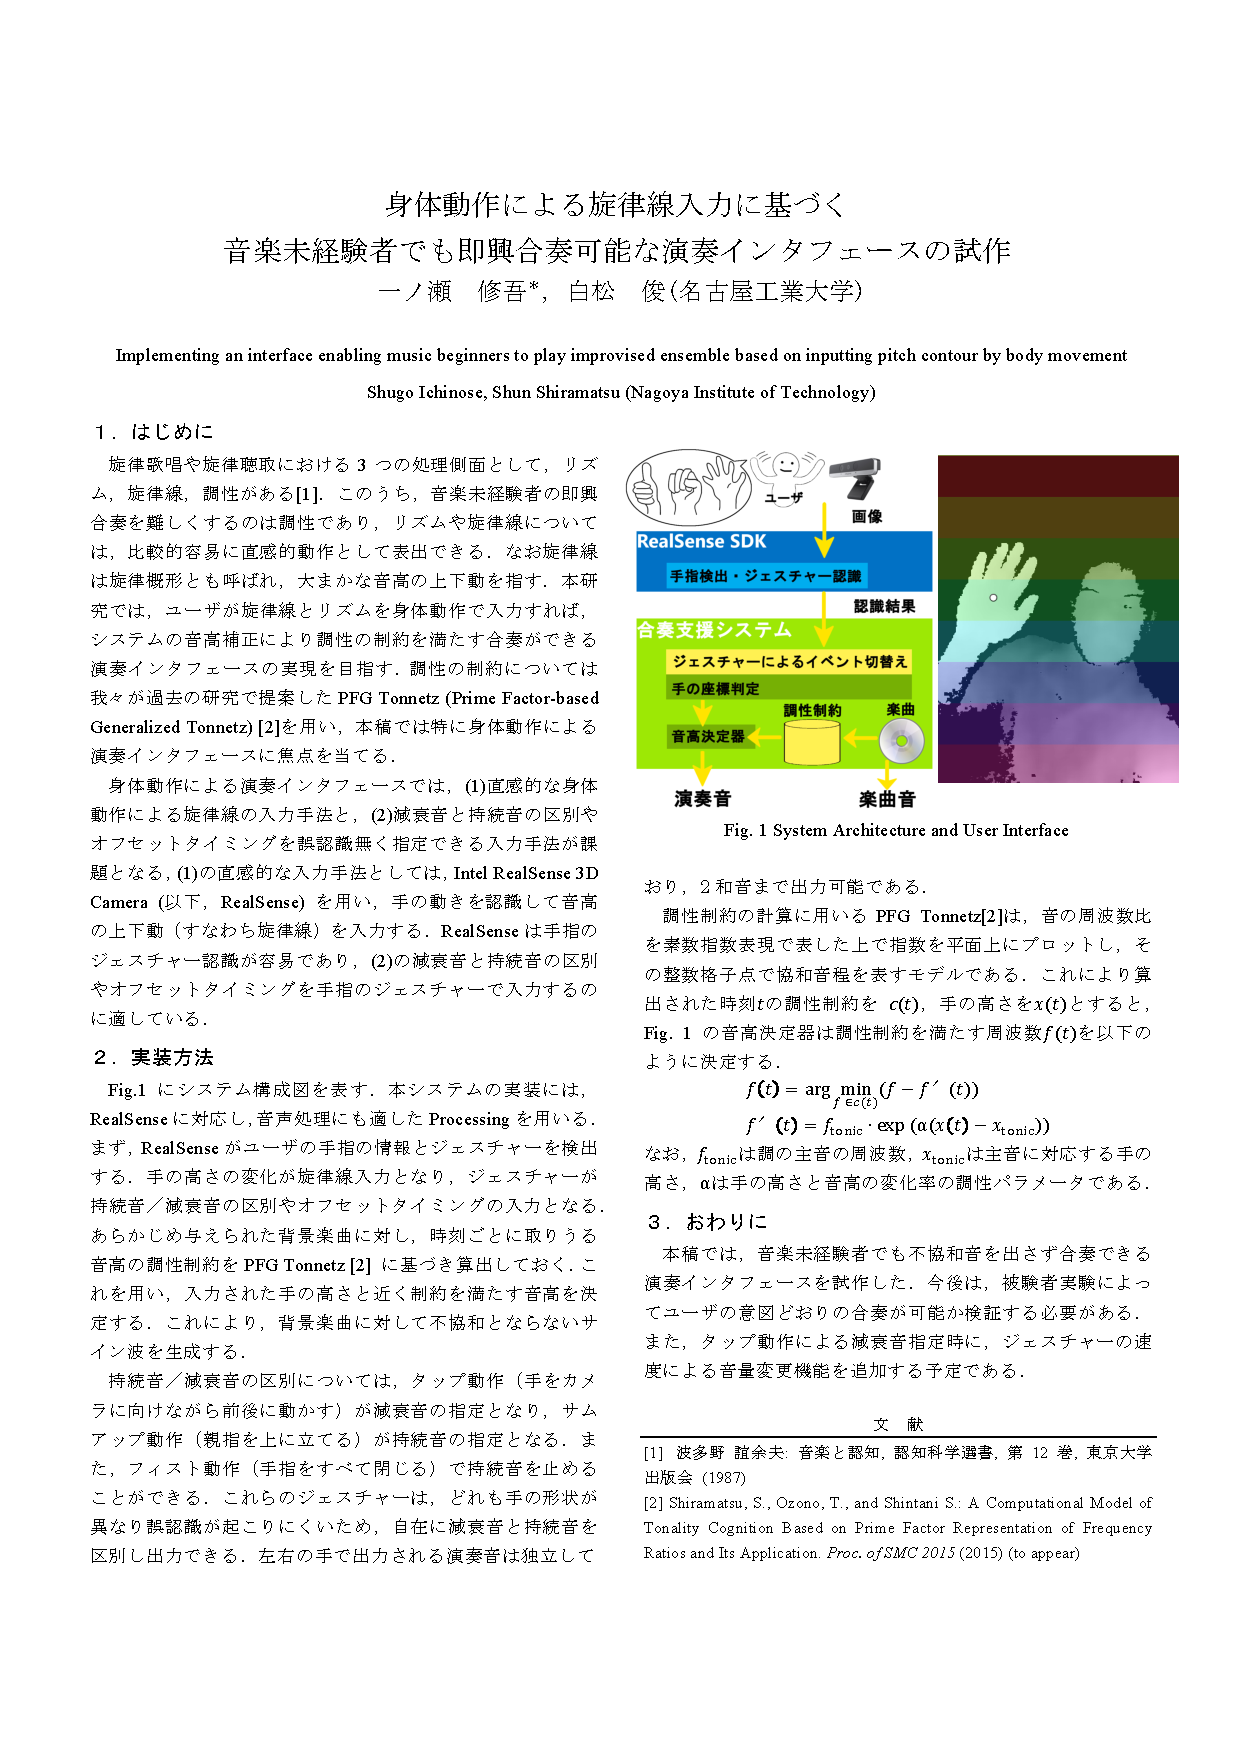
\includegraphics[width=1.0\linewidth]{assets/pdf/ichinose2015tokai0717.pdf}
    \end{center}
\end{figure}

\clearpage

\cleardoublepage

% タイトル
%!TEX root = ../../main.tex
% タイトルページ
%\documentclass[a4j,12pt]{jreport}
%\usepackage{graphicx}
%\usepackage{times}
%\usepackage{selectp}
%\usepackage{epsf}
%\usepackage{epsbox}
%\usepackage{graphicx}
%\usepackage{verbatimfiles}
%\usepackage{here}
%%\usepackage{url}
%\usepackage{fancyhdr}
%\usepackage{algorithm}
%\usepackage{cite}
%\usepackage{ascmac}
%\usepackage{amsmath}
%\usepackage{amsthm}
%\usepackage{amssymb}
%\usepackage{latexsym}

%\usepackage{thesis}
%\input{mymacros}

%\oddsidemargin=17mm
%\evensidemargin=-4mm

%\setlength{\textwidth}{40zw}
%\begin{document}

\thispagestyle{empty}
\setcounter{page}{0}

%%%%%%%%%%%%%%%%%%%%%%%%%%%%%%%%%%%%%%%%%%%%%%%%%
% 定義
%%%%%%%%%%%%%%%%%%%%%%%%%%%%%%%%%%%%%%%%%%%%%%%%%

% タイトル
\def \title{MissionForest: 組織内外における\\協働支援のためのタスク構造化システムの試作}

% 著者
\def \author{後藤~誉昌}

% 提出日
\def \date{\today}

% 指導教官名
\def \teacher{白松~俊}

% 指導教官の肩書き
\def \teacherrank{准教授}

% 所属
\def \belong{名古屋工業大学\\工学部 情報工学科}

% 入学年度
\def \year{23}

% 学籍番号
\def \regnum{24115054}

%%%%%%%%%%%%%%%%%%%%%%%%%%%%%%%%%%%%%%%%%%%%%%%%%
% 本文
%%%%%%%%%%%%%%%%%%%%%%%%%%%%%%%%%%%%%%%%%%%%%%%%%

\def\sizeLL#1{\Huge #1}
\def\sizeL#1{\LARGE #1}
\def\sizeM#1{\Large #1}
\def\sizeS#1{\large #1}

\def\REYrule{\hbox to 5cm{\leaders\hrule height 1pt\hfill}}
\newbox\REYbox
\def\announce#1{
  \setbox\REYbox=\hbox{\REYrule\quad{\Large\bf #1}\quad\raise3pt\REYrule}%
  \gdef\REYbigrule{\hbox to \wd\REYbox{\leaders\hrule height 1pt \hfill}}%
  \centerline{\raise3pt\REYrule\vspace*{2mm}\quad{\LARGE #1}\quad\raise3pt\REYrule}}
\def\endannounce{\par\centerline{\REYbigrule}}

\begin{titlepage}
 \begin{center}
 %\renewcommand{\baselinestretch}{1.0}
  \vspace*{5mm}
  \sizeLL{卒業論文}\\
  \vspace*{10mm}
  \begin{announce}{(題~~目)}
   \sizeL{\title}\\
  \end{announce}
  \vspace*{20mm}
  \sizeM{指導教員~~~~~}\sizeL{\teacher}\sizeM{~~\teacherrank}\\
  %\vspace*{40mm} % 題目が2行の場合
 % \vspace*{30mm} % 題目が3行の場合
 \vspace{10mm}
  \sizeM{\belong}\\
  \vspace*{10mm}
  \sizeM{平成 \year 年 4 月 入学}\\
  \vspace*{3mm}
  \begin{table}[H]
    \begin{center}
     \begin{tabular}{cl}
      \sizeM{(学籍番号)} & \sizeL{{\underline{~~ \regnum ~~}}} \\
      \sizeM{(氏~名)} & \sizeL{\underline{~~ \author ~~}} \\
     \end{tabular}
    \end{center}
   \end{table}
  \vspace*{10mm}
  \sizeS{(提出日:~\today)}
  % \sizeS{(提出日:\ ~平成28年2月8日)}
 \end{center}
\end{titlepage}

%\end{document}


\end{document}
